\section*{Parte 1}\label{sec:parte1}
\subsection*{Introdução}
Na primeira parte do trabalho realizado, foi efetuado uma recolha dos dados localizados na \textit{Pluggable Database} e \textit{Root Database} em \textit{Java}, com o objetivo de monitorizar a performance de uma nova base de dados \textit{oracle} concebida pelos elementos do grupo, com a informação levantada respetivamente. Nesta secção, efetuaremos uma breve explicação acerca de todas as classes criadas, a conexão á base de dados e do conjunto de queries realizadas que permitem a reunião da informação pretendida.

\subsection*{Ligação à Base de Dados}
A conexão á base de dados solicitada, é realizada por intermédio da driver JDBC. A \textit{Java Database Connectivity}, permite o envio de queries através de um objeto \textit{statement} recolhendo de igual forma os resultados das mesmas. Desta forma, é possível o armazenamento da informação em estruturas de dados apropriadas para a criação da nova DB.
\begin{lstlisting}
    try {
        Class.forName("oracle.jdbc.driver.OracleDriver");
    } catch (ClassNotFoundException e) {
        System.out.println("Where is your Oracle JDBC Driver?");
        e.printStackTrace();
        return;
      }
        Connection connection = null;
    try {
        // Exemplo de conexao: pluggable db.
        connection =DriverManager.getConnection("jdbc:oracle:thin:@localhost:1521/orcl", "system", "oracle");
    } catch (SQLException e) {
        System.out.println("Connection Failed! Check output console");
        e.printStackTrace();
        return;
      }
    if (connection != null) {
        System.out.println("Connected to database");
    } else {
        System.out.println("Failed to make connection!");
      }
    // Criacao da statement.
    Statement stnt = connection.createStatement();
    // Execucao da query e recolha do resultado.
    ResultSet tablespaces = stnt.executeQuery(...);~

\end{lstlisting}
\vspace{5mm}
\begin{figure}[h!]
 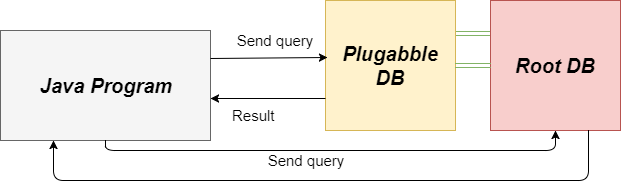
\includegraphics[width=\linewidth]{tex/figs/esquema.png}
    \caption{Figura que representa o esquema de funcionamento da recolha de dados.} 
    \label{fig:esquema1}
\end{figure}
\subsection*{\textit{Tablespaces}}
Um banco de dados é dividido em uma ou mais unidades de armazenamento lógico chamadas de \textit{Tablespaces}. Através da \textit{Pluggable DB} onde se encontra toda a sua estrutura, decidimos retirar os seguintes dados uma vez que, achamos que constituem o essencial a extrair para uma futura monitorização da sua informação:
\begin{itemize}
    \item Espaço utilizado.
    \item Espaço livre.
    \item Percentagem de espaço utilizado
	\item Tamanho Máximo(Espaço ocupado por todos os \textit{tablespaces}).
\end{itemize}
De forma a cumprir os pontos acima listados, foi necessária a criação de uma classe \textit{\textbf{Tablespaces.java}} que guarda os dados extraídos.
Após estabelecer a conexão á base de dados \textit{orcl(pluggable db)}, é executada a seguinte query:
\vspace{2mm}
\begin{lstlisting}
        ResultSet tablespaces = stnt.executeQuery(
        "select fs.tablespace_name,(df.totalspace - fs.freespace),fs.freespace ,df.totalspace, round(100 * (fs.freespace / df.totalspace)) 
        from" +
         " (select tablespace_name,round(sum(bytes) / 1048576) TotalSpace from dba_data_files group by tablespace_name) df," +
         " (select tablespace_name,round(sum(bytes) / 1048576) FreeSpace from dba_free_space group by tablespace_name) fs" +
       "where df.tablespace_name = fs.tablespace_name");
     
\end{lstlisting}
\vspace{2mm}
A query apresentada, devolve a informação pretendida consultando as \textit{views} relativas aos \textit{datafiles dba data files e dba free space}. O \textit{dba data files} compreende toda a informação acerca do \textit{datafile} incluindo, o \textit{tablespace} a que está associado onde o \textit{dba free space}, apresenta as componentes com espaço vazio no \textit{datafile}.

Para cada resposta recebida proveniente da base de dados em questão, é criada um objeto \textit{Tablespace} que reúne toda esta informação. O objeto é posteriormente guardado numa lista de \textit{Tablespaces} para uma fácil e futura utilização:
\vspace{2mm}
\begin{lstlisting}
while(tablespaces.next()){
    @SuppressWarnings("UnusedAssignment")
    Tablespaces t = new Tablespaces();
    t = new Tablespaces(tablespaces.getString(1),
    tablespaces.getInt(3),tablespaces.getInt(2),
    tablespaces.getFloat(5),tablespaces.getInt(4));
    list_tablespaces.add(t);
}
\end{lstlisting}
\subsection*{\textit{Datafiles}}
Cada \textit{Tablespace} numa \textit{Oracle Database}, consiste em um ou mais ficheiros chamados de \textit{Datafiles}. Estes compreendem estruturas físicas conforme o sistema operativo na qual o Oracle está a correr. Toda a data, está coletivamente guardada em \textit{Datafiles} que  constituem cada \textit{Tablespace} da base de dados. 
Neste presente trabalho, decidimos guardar a seguinte informação acerca dos \textit{Datafiles}, da base de dados em questão, que se encontra descrita nos seguintes pontos e, na nossa opinião, descrevem o essencial a retirar de cada \textit{Datafile}:
\begin{itemize}
    \item Espaço livre.
    \item Espaço que ocupa.
    \item Espaço utilizado.
    \item Percentagem de espaço utilizado.
    \item \textit{Tablespace} a que está associado.
\end{itemize}
Em primeiro lugar, tal como efetuado para os \textit{Tablespaces}, criamos uma classe para guardar os dados extraídos em relação aos \textit{Datafiles}: \textit{\textbf{Datafiles.java}}. A base de dados utilizada foi a \textit{Pluggable DB} e após efetuada a conexão, executamos a seguinte query para receber dela o conjunto de informação pretendida:
\begin{lstlisting}
 ResultSet datafiles = stnt.executeQuery("SELECT  Substr(df.tablespace_name,1,20) \"Tablespace Name\",\n" +
"        Substr(df.file_name,1,80) \"File Name\",\n" +
"        Round(df.bytes/1024/1024,0) \"Size (M)\",\n" +
"        decode(e.used_bytes,NULL,0,Round(e.used_bytes/1024/1024,0)) \"Used (M)\",\n" +
"        decode(f.free_bytes,NULL,0,Round(f.free_bytes/1024/1024,0)) \"Free (M)\",\n" +
"        decode(e.used_bytes,NULL,0,Round((e.used_bytes/df.bytes)*100,0)) \"% Used\"\n" +
"FROM    DBA_DATA_FILES DF,\n" +
"       (SELECT file_id,\n" +
"               sum(bytes) used_bytes\n" +
"        FROM dba_extents\n" +
"        GROUP by file_id) E,\n" +
"       (SELECT Max(bytes) free_bytes,\n" +
"               file_id\n" +
"        FROM dba_free_space\n" +
"        GROUP BY file_id) f\n" +
"WHERE    e.file_id (+) = df.file_id\n" +
"AND      df.file_id  = f.file_id (+)\n" +
"ORDER BY df.tablespace_name,\n" +
"         df.file_name");
\end{lstlisting}
\vspace{2mm}
Esta query consulta as views de \textit{dba data files, dba extents e dba free space}. O \textit{dba data files} contêm a informação sobre o \textit{datafile} incluindo o seu nome e o \textit{tablespace} a que está associado. O \textit{dba free space} compreende todos os dados sobre as componentes com espaço vazio no \textit{datafile}.\textit{Dba extents} descreve as extensões que compõem os segmentos em todos os espaços de tabelas na base de dados. São selecionados dessa \textit{view} o numero de bytes usados pelo \textit{datafile}  e o id do ficheiro respetivo.

Por cada resposta recebida proveniente da base de dados, é consultada a lista previamente criada para guardar toda a informação dos \textit{Tablespaces}. Para cada \textit{tablespace} encontrado na lista se o seu nome for igual ao recebido, guarda-se o seu objeto juntamente com a informação recolhida do \textit{datafile}  associado e é criado um objeto \textit{Datafile} para esse efeito. Por último, cada objeto \textit{Datafile} é guardado numa lista de \textit{datafiles} com a finalidade de extrair facilmente o seu conteúdo de modo a realizar uma futura monitorização dos seus dados:
\vspace{2mm}
\begin{lstlisting}
while(datafiles.next()){
           
    Tablespaces tb = null;
    for (int i = 0 ; i < list_tablespaces.size() ; i++){
        tb = list_tablespaces.get(i);
        if(tb.getName().equals(datafiles.getString(1)))
            break;
    }
    Datafiles d = new Datafiles(tb,datafiles.getString(2),datafiles.getInt(5),
    datafiles.getInt(3),datafiles.getInt(4),datafiles.getFloat(6);
    list_datafiles.add(d);
} 
\end{lstlisting}
\subsection*{Users}
A base de dados é acedida por um conjunto de \textit{Users}. De forma a reunir toda a informação sobre \textit{users}, extraímos os dados contidos nos seguintes pontos que achamos ser o essencial a retirar:
\begin{itemize}
    \item \textit{Default tablespace} associado ao \textit{user}.
    \item \textit{Temporary tablespace} associado ao \textit{user}.
    \item \textit{Quota} em \textit{bytes} dos \textit{tablespaces}.
    \item \textit{Status} da conta do utilizador.
    \item Previlégio do utilizador concedido pelo sistema.
    \item Informação do tipo de utilizador(eg: ativo).
    \item \textit{CPU usage} do utilizador respetivo.
\end{itemize}
Em primeiro lugar, estabelecemos a conexão á \textit{Pluggable DB} pois, os dados listados encontram-se armazenados nessa base de dados. Criamos uma classe \textbf{\textit{Users.java}} que guarda toda esta informação. Após efetuada a conexão, efetuamos a seguinte query:
\vspace{2mm}
\begin{lstlisting}
 ResultSet users = stnt.executeQuery("select username, default_tablespace, temporary_tablespace, account_status 
 from dba_users");
\end{lstlisting}
\vspace{2mm}
A query exibida consulta a view \textit{dba users}. A \textit{dba users}, apresenta todos os utilizadores da base de dados. A partir da mesma, é possivel extrair o nome, a \textit{default tablespace}, a \textit{temporary tablespace} e o \textit{status} da conta do utilizador.

Para cada resposta recebida no envio desta query, é criado um objeto \textit{User} que armazena os dados e posteriormente é adicionado a uma lista \text{Users} para uma fácil organização e futura monitorização:
\vspace{2mm}
\begin{lstlisting}
while(users.next()){
    @SuppressWarnings("UnusedAssignment")
    Users u = new Users();
    u = new Users(users.getString(1),users.getString(2),
    users.getString(3), users.getString(4));
    list_users.add(u);
}
\end{lstlisting}
\vspace{2mm}
De seguida, é executada uma nova query:
\vspace{2mm}
\begin{lstlisting}
 ResultSet user_quota = stnt.executeQuery("select username, tablespace_name, bytes from dba_ts_quotas");
\end{lstlisting}
\vspace{2mm}
A query exibida consulta a view \textit{dba ts quotas}. É possível então extrair o nome do \text{tablespace} associado ao utilizador respetivo assim como, o número de bytes da quota nesse \textit{tablespace}. 

Para cada resposta recebida sobre a query em questão, percorre-se todos os objetos \textit{User} guardados na lista de \textit{Users} e verifica-se se o nome do user selecionado corresponde a um deles. Se corresponder, adiciona-se a nova informação extraída a esse objeto:
\vspace{2mm}
\begin{lstlisting}
 while(user_quota.next()){
    int result = 0;
    Users u = null;
    for (int i = 0 ; i < list_users.size() ; i++){
        u = list_users.get(i);
        if(u.getUser().equals(user_quota.getString(1))){
            result = 1;
            break;
        }
    }
    if(result == 1)
    { 
        u.setTabName(user_quota.getString(2));
        u.setQb(user_quota.getInt(3));
    }  
}
\end{lstlisting}
\vspace{2mm}
Logo depois, realiza-se uma nova query:
\vspace{2mm}
\begin{lstlisting}
  ResultSet user_priv = stnt.executeQuery("select grantee, privilege from dba_sys_privs");
\end{lstlisting}
\vspace{2mm}
A query apresentada consulta a view \textit{ dba sys privs}. Esta view descreve os privilégios e \textit{roles} concedidos aos utilizadores pelo sistema. Desta forma, é possível extrair a informação sobre o privilégio do utilizador em questão.

Para cada resposta recebida, percorre-se todos os objetos \textit{User} guardados na lista de \textit{Users} e verifica-se se o nome do user selecionado corresponde a um deles. Se corresponder, adiciona-se a nova informação extraída a esse objeto:
\vspace{2mm}
\begin{lstlisting}
while(user_priv.next()){
             
    int result = 0;
    Users u = null;
    for (int i = 0 ; i < list_users.size() ; i++){
        u = list_users.get(i);
        if(u.getUser().equals(user_priv.getString(1))){
            result = 1;
            break;
        }
    }
    if(result == 1){ u.setPriv(user_priv.getString(2));}  
}
\end{lstlisting}
\vspace{2mm}
Por fim, concretizada a seguinte query:
\vspace{2mm}
\begin{lstlisting}
ResultSet active_user = stnt.executeQuery("SELECT\n" +
"   s.username,\n" +
"   t.sid,\n" +
"   s.serial#,\n" +
"   SUM(VALUE/100) as \"cpu usage (seconds)\"\n" +
"FROM\n" +
"   vsession s,\n" +
"   vsesstat t,\n" +
"   vstatname n\n" +
"WHERE\n" +
"   t.STATISTIC# = n.STATISTIC#\n" +
"AND\n" +
"   NAME like '%CPU used by this session%'\n" +
"AND\n" +
"   t.SID = s.SID\n" +
"AND\n" +
"   s.username is not null\n" +
"GROUP BY username,t.sid,s.serial#");
\end{lstlisting}
\vspace{2mm}
A query exibida consulta 3 views: \textit{v session, v sesstat, vstatname}. A \textit{vsession}, lista as informações da sessão para cada sessão atual. A \textit{v sesstat}, apresenta as estatísticas da sessão do usuário. A \textit{vstatname}, exibe nomes estatísticos descodificados para as estatísticas mostradas nas tabelas \textit{v sesstat e v sysstat}. Em conjunto é possível extrair a usagem de \textit{CPU} do utilizador respetivo.

Para cada resposta recebida, percorre-se todos os objetos \textit{User} guardados na lista de \textit{Users} e verifica-se se o nome do user selecionado corresponde a um deles. Se corresponder, adiciona-se a nova informação extraída a esse objeto:
\vspace{2mm}
\begin{lstlisting}
while(active_user.next()){
           
    int result = 0;
    Users u = null;
    for (int i = 0 ; i < list_users.size() ; i++){
        u = list_users.get(i);
        if(u.getUser().equals(active_user.getString(1))){
            result = 1;
            break;
        }
    }
    if(result == 1){
        u.setSid(active_user.getString(2));
        u.setSerial(active_user.getString(3));
        u.setCPU(active_user.getString(4));
    }    
}
\end{lstlisting}
\vspace{2mm}
\subsection*{Tables}
As \textit{Tables} são a unidade básica de armazenamento de dados numa base de dados \textit{Oracle}. Decidimos extrair os seus  dados descritos nos seguintes pontos pois, achamos que é o essencial a retirar das \textit{Tables}:
\begin{itemize}
    \item Tabelas mais acedidas.
    \item Tabelas com o número maior de registos.
    \item Tabelas apagadas.
\end{itemize}
Toda a informação sobre \textit{Tables} encontra-se registada na \textit{Pluggable DB}. De modo a reunir todos os dados provenientes da mesma, criamos a classe \textbf{\textit{Tables.java}}. Após efetuada a conexão, executamos em primeiro lugar a seguinte query:
\vspace{2mm}
\begin{lstlisting}
ResultSet tables = stnt.executeQuery("select table_name,dropped,tablespace_name,
num_rows from dba_tables ORDER BY num_rows");
\end{lstlisting}
\vspace{2mm}
A query exibida consulta a tabela \textit{dba tables}. A \textit{dba tables}, descreve todas as tabelas relacionais na base de dados. Desta retiramos o nome da tabela, a flag que indica se foi apagada ou não, o nome do \textit{tablespace} a que está associada e o número de registos.

Para cada resposta recebida do envio da query em questão,
criamos um objeto \textit{Tables} que reúne toda a informação. Realizamos uma procura pelos objetos \texttit{Tablespace} na lista de \textit{Tablespaces}. Se o nome do objeto encontrado for igual ao recebido, então é adicionado os seus dados ao objeto \texttit{Tables} em questão. Posteriormente esse objeto é guardado numa lista de \textit{Tables} com o propósito de facilitar na extração dos dados de cada um dos elementos da lista:
\vspace{2mm}
\begin{lstlisting}
while(tables.next()){
    @SuppressWarnings("UnusedAssignment")
    Tables tb = new Tables();
    tb = new Tables(tables.getString(1),
    tables.getString(2),tables.getInt(4));
    for (int i = 0 ; i < list_tablespaces.size() ; i++){
        @SuppressWarnings("UnusedAssignment")
        Tablespaces t = null;
        t = list_tablespaces.get(i);
        if(t.getName().equals(tables.getString(3))){
            tb.setTable(t);
            break;
        }
    }
    list_tables.add(tb);
}
\end{lstlisting}
\vspace{2mm}
De seguida, é realizada uma nova query:
\vspace{2mm}
\begin{lstlisting}
 ResultSet tables_access =  stnt.executeQuery("SELECT t.owner, t.table_name, lr.VALUE + pr.VALUE AS total_reads\n" +
"FROM (SELECT	owner, object_name, VALUE\n" +
"FROM	vsegment_statistics\n" +
"WHERE	statistic_name = 'logical reads') lr, (SELECT owner, object_name, VALUE\n" +
"FROM	vsegment_statistics\n" +
"WHERE	statistic_name = 'logical reads') pr, dba_tables t\n" +
"WHERE lr.owner = pr.owner AND lr.object_name = pr.object_name AND lr.owner = t.owner AND lr.object_name = t.table_name\n" +
"ORDER BY 3 desc");
\end{lstlisting}
\vspace{2mm}
A query apresentada consulta a view \textit{segment statistics}. Esta exibe informações sobre estatísticas de nível de segmento. É utilizada para obter informação sobre o número de acessos ás tabelas em questão.

Para cada resposta recebida, é consultada a lista previamente criada de \textit{tables} e para cada objeto, verifica se o nome da tabela recebida é igual ao nome da sua tabela. Se for igual, é adicionada a informação sobre o número de acessos:
\vspace{2mm}
\begin{lstlisting}
 while(tables_access.next()){
    for (int i = 0 ; i < list_tables.size() ; i++){
        @SuppressWarnings("UnusedAssignment")
        Tables t = null;
        t = list_tables.get(i);
        if(t.getName().equals(tables_access.getString(2))){
            t.setNA(tables_access.getInt(3));
            break;
        }
    }
}
\end{lstlisting}
\subsection*{\textit{Sessions}}
Um utilizador conecta-se a uma base de dados a partir de 1 ou mais \textit{sessions}. A \textit{Pluggable DB} concentra todos os dados relativos a estas. De modo a reunir a informação sobre \textit{sessions}, é necessário reunir os pontos mais importantes a extrair. Portanto, aqui se encontra a informação a retirar:
\begin{itemize}
    \item \textit{User} associado á \textit{session}.
    \item \textit{Schema Name} da \textit{session}.
    \item \textit{Login time} na qual foi iniciada a \textit{session}.
\end{itemize} 
De forma a reunir a informação proveniente da \textit{Pluggable DB}, criamos a classe \textbf{\textit{Sessions.java}} que guarda os dados relativos á sessão. Após efetuada a conexão, executamos a seguinte query de forma a extrair o pretendido:
\vspace{2mm}
\begin{lstlisting}
ResultSet session =  stnt.executeQuery("SELECT UserName, SchemaName, Logon_Time\n" +
"FROM V$Session\n" +
"WHERE\n" +
"Status='ACTIVE' AND\n" +
"UserName IS NOT NULL");

\end{lstlisting}
\vspace{2mm}
A query apresentada consulta a \textit{view} \textit{Session}. Esta \textit{view} contêm todos as informações sobre a sessão respetiva incluindo o nome do \textit{user} , do \textit{schema} e o tempo do \textit{login}.

Para cada query enviada, é recebida a informação sobre a \textit{session} que é posteriormente guardada numa lista de \textit{sessions}. Cada objeto \textit{session} compreende a informação previamente listada. Além disso, para cada resposta recebida, é realizada uma procura na lista de \textit{users} anteriormente criada. Se o nome do \textit{user} for igual ao nome recebido então o objeto \textit{User} encontrado, é incluido na informação do objeto \textit{Session} sendo então guardado na lista de \textit{sessions}:
\vspace{2mm}
\begin{lstlisting}
while(session.next()){
    for (int i = 0 ; i < list_users.size() ; i++){
        @SuppressWarnings("UnusedAssignment")
        Users u = null;
        u = list_users.get(i);
        if(u.getUser().equals(session.getString(1))){
            Sessions s = new Sessions(u,session.getString(2),session.getString(3));
            list_sessions.add(s);
            break;
        }
    }
}
\end{lstlisting}
\subsection*{\textit{Memory}}
Um dos fatores mais importantes no nosso objetivo de criar uma nova base de dados a partir dos dados recolhidos, consiste na \textit{memory} respetiva. É importante então, averiguar e extrair os seguintes pontos em relação á mesma:
\begin{itemize}
    \item Memória utilizada.
	\item Memoria livre.
	\item Percentagem memória utilizada.
\end{itemize}
As informação sobre \textit{memory} encontra-se na Root DB. Após efetuar a conexão, em primeiro lugar, é necessário criar uma classe para guardar os dados da \textit{memory}: \textbf{\textit{Memory.java}}. De seguida, executa-se a seguinte query:
\vspace{2mm}
\begin{lstlisting}
ResultSet sga = stnt.executeQuery("select (sga+pga)/1024/1024 as \"sga_pga\"\n" +
"from \n" +
"(select sum(value) sga from v$sga),\n" +
"(select sum(pga_used_mem) pga from v$process)");
}
\end{lstlisting}
\vspace{2mm}
A query apresentada, consulta as views de \textit{sga e process}. A view \textit{sga}, exibe informações resumidas sobre a área global do sistema devolvendo o somatório de \textit{value} que corresponde á memoria total do sistema. A view \textit{process}, mostra toda a informação sobre processos ativos. Esta devolve o somatório da \textit{pga used mem}, que significa o total da memória atualmente utilizada pelos processos. Em conjunto com a view \textit{sga}, devolve a memória total:
\vspace{2mm}
\begin{lstlisting}
double total = 0;
while(sga.next()){
            total = sga.getDouble(1);
}
\end{lstlisting}
\vspace{2mm}
De seguida,foi executada a seguinte query:
\vspace{2mm}
\begin{lstlisting}
ResultSet sga2 = stnt.executeQuery("select sum(bytes)/1024 from v sgastat where name = 'free memory'");
\end{lstlisting}
\vspace{2mm}
A query exibida consulta a view \textit{sgastat}. Esta dispõe de informações detalhadas sobre a área global do sistema devolvendo o somatório em bytes da memory livre. Para cada resposta do envio da query em questão,  é criado um novo objeto \textit{Memory} com o total de bytes da memoria utilizada a partir da query anterior, o total de bytes de memória livre(não utilizada) e por fim a percentagem de bytes livres:
\vspace{2mm}
\begin{lstlisting}
while(sga2.next()){
    double bytes = sga2.getDouble(1)/1024;
    m = new Memory(total,bytes,bytes/total); 
}
\end{lstlisting}
\vspace{2mm}
\subsection*{I/O}
Nesta subsecção, concentramo-nos na extração de informação sobre as leituras e escritas físicas realizadas ao disco. Para tal, necessitamos de realizar a conexão á \textit{Root DB} visto que, é a partir desta que será possível obter os dados pretendidos. Para a leitura física dos dados no disco foi criada a classe:\textbf{\textit{IOReads.java}} e \textbf{\textit{IOWrites.java}} para as escritas físicas. De seguida e em primeiro lugar , realiza-mos a seguinte query:
\vspace{2mm}
\begin{lstlisting}
 ResultSet ioreads = stnt.executeQuery("select metric_name,begin_time,end_time,value from v sysmetric_history "
 + "where metric_name = 'Physical Reads Per Sec' order by begin_time");
\end{lstlisting}
\vspace{2mm}
A query apresentada consulta a view de \textit{sysmetric history}. Esta view exibe todos os valores de métricas do sistema disponíveis na base de dados. Devolve o nome da metrica, o tempo de inicio e final de leitura física ao disco por segundo e o valor da métrica. É criada um objeto \textit{IOReads} por cada resposta ao envio desta query de forma a guardar os dados apresentados. No final, cada um destes objetos é enviado para uma lista de \textit{IOReads} para uma fácil e futura monitorização:
\vspace{2mm}
\begin{lstlisting}
while(ioreads.next()){
    IOReads r = new IOReads(ioreads.getString(1),ioreads.getString(2), ioreads.getString(3),ioreads.getDouble(4));
    io_reads.add(r);
}
\end{lstlisting}
\vspace{2mm}
Em segundo lugar, é executada a seguinte query:
\vspace{2mm}
\begin{lstlisting}
ResultSet iowrites = stnt.executeQuery("select metric_name,begin_time,end_time,value from v sysmetric_history "
+ "where metric_name = 'Physical Writes Per Sec' order by begin_time");
\end{lstlisting}
\vspace{2mm}
A query exibida consulta a view \textit{sysmetric history}. Devolve os mesmos dados que a query anterior apenas diferencia no \textit{metric name} onde esta devolve os dados relativos ás escritas fisicas no disco por segundo. É criado um objeto \textit{IOWrites} por cada resposta obtida de forma a guardar os dados. No final, cada um destes objetos é enviado para uma lista de \textit{IOWrites} para simplificar o modo como são criados os schemas no capítulo seguinte:
\vspace{2mm}
\begin{lstlisting}
while(iowrites.next()){
    IOWrites w = new IOWrites(iowrites.getString(1),iowrites.getString(2), iowrites.getString(3),iowrites.getDouble(4));
    io_writes.add(w);
}
\end{lstlisting}